\section{Live Auditing}
\label{sec:live-audit}

Section~\ref{sec:retro-results} showed the effectiveness of applying
the balance invariant on restropective data to accurately identify
past bridge attacks.  Incorporating the logic used in the
retrospective analysis, we implemented a real-time auditing system
that uses the balance invariant to monitor ongoing transactions on a
bridge.

Since most of the bridges in our retrospective analysis are shut down at
the time of writing (Figure~\ref{fig:bridge-timeline}), we focus on the
Wormhole bridge.  Wormhole is still operational, supports a wide
variety of blockchains, and is among the most popular bridges in terms
of transaction activity~\cite{zhang2023sok}.  This live system
monitors thousands of withdrawal transactions per day across ten
blockchains, which together account for 60\% of all withdrawal
transactions on Wormhole.  Extending the system to support other
bridges is straightforward.

%% Incorporating the methodology described in Section~\ref{sec:meth}, we
%% implement a real-time auditing system for Wormhole. This live system
%% monitors thousands of withdrawal transactions per day across the 10
%% blockchains, which together account for around 60\% of all withdrawal
%% transactions on Wormhole. 
%% %
%% We first describe the system architecture and implementation, and then
%% its deployment.

%% Below, we start by describing the architecture of our live auditing
%% system, followed by X and Y. \alex{missing: augmenting w/
%%   Wormholescan}


\subsection{System Overview}

Figure~\ref{fig:live-audit-arch} depicts the architecture of our live
auditing system. The system consists of three main components. The
\textit{Blockchain Monitor} tracks the blockchain network and
retrieves the latest deposit and withdrawal transactions. The
\textit{Auditor} checks extracted transactions for invariant
violations. The \textit{Database} component stores all the
transactions and auditing results.

% [covered by the Open Science Policy blurb]
% (We will make the code publicly available upon publication.)

\begin{figure}[t]
\centering
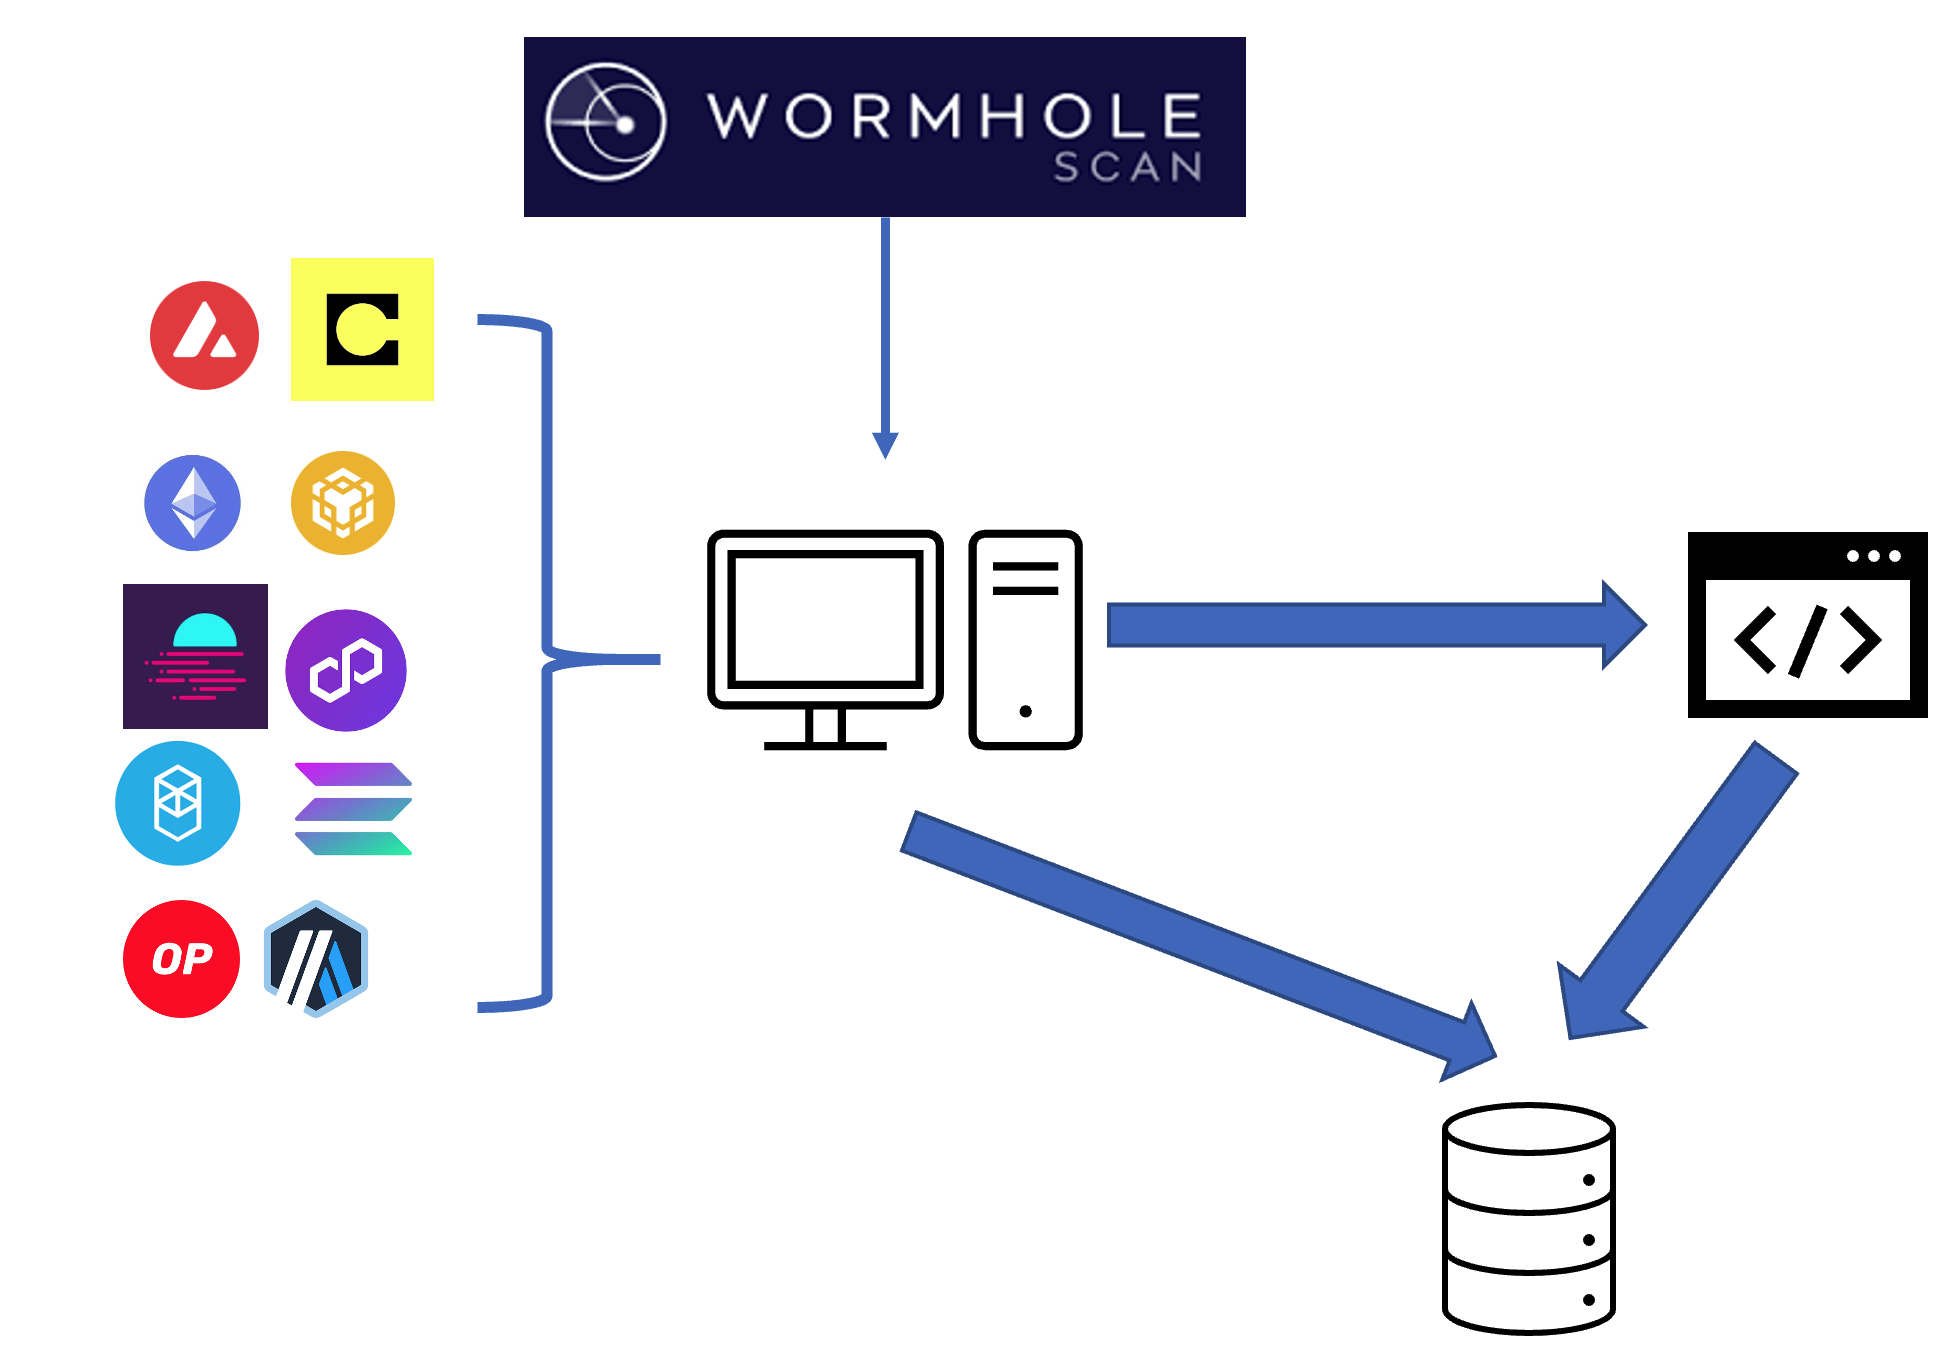
\includegraphics[width=\columnwidth]{fig/dbarch.pdf}
\caption{Live auditing system which consists of three components.}
\label{fig:live-audit-arch}
\end{figure}

%\subsection{Blockchain Monitor}
\textbf{Blockchain Monitor.}
%
The Blockchain Monitor obtains deposit and withdrawal transactions by
periodically retrieving the latest finalized blocks.  The Monitor
% primarily
uses the same commercial RPC services for collecting
Wormhole deposits and withdrawals as we used for the retrospective
analysis (Section~\ref{sec:retro-data}).\footnote{A fully operational
deployment would manage nodes participating in each of the blockchains
to obtain transactions in block data directly.}
%% However, this data
%% is not complete since a withdrawal transaction may reference a deposit
%% on a blockchain not supported by our system or pre-dates our data
%% collection (although infrequent, withdrawals do occur many months
%% after the deposit). To audit withdrawals like these, our system
%% retrieves their corresponding deposit transactions using Wormholescan, a
%% service maintained by Wormhole that indexes bridge
%% transactions. Wormholescan allows us to audit withdrawal transactions
%% whose corresponding deposits are not indexed by our system, improving
%% our audit coverage.\footnote{We note that Wormholescan occasionally
%% returns an error when queried for valid withdrawal transactions, as it
%% focuses on completeness on deposits since users need deposits
%% acknowledged to then trigger withdrawals. We have filed a bug report
%% with Wormhole.}
%% \deian{I would make clear if we actually need Wormholescan to be trustwhorthy or
%% not. I don't think we actually do (but later we bork) so worth clarifying (it
%% only really matters for availability). I would also prefix the Wormholescan
%% bit by saying the RC providers don't let you access ``very old'' events. And I
%% would end this discusison by saying that in practice you would run your own node
%% (which will let you query whatever you want however far back you want).}

% We also note that
The Monitor only retrieves finalized blocks since unfinalized blocks
may be reverted or reordered.  Since different blockchains have
different finality times, we use the timestamp of the latest finalized
block of Ethereum as the synchronization time since Ethereum has the
slowest finality time (around 12 minutes)~\cite{Finality:online}.
%% \footnote{Different systems may have thresholds for
%% finality, but usually wait for at least a few minutes.}
% We leave it to future work to explore how to synchronize to real time.
%% \elisa{It not super clear what the difference between the
%%   synchronization time (15 min) and the refresh time is. So with a
%%   sync time of 15, every time we audit, we are actually 15+10min
%%   behind?}
After retrieving the blocks, the Monitor extracts deposit and
withdrawal transactions for Wormhole and saves them to a local
database.

The polling interval is configurable and the Monitor polls chains
every 1 minute by default.  As a result, the live auditing system is
as recent as the polling interval combined with the finality time
--- a situation similar to bridges due to the polling nature of
distributed off-chain communication.
% We leave it to future work to optimize the delay further.

%% \alex{move wormholescan here.}

%% \geoff{this is the main effort because it needs to be extended for
%%   every chain that we want to audit?  this is where we should say that
%%   we monitor 11 chains (and name at least the popular ones), and
%%   something about why we don't monitor all chains supported by
%%   Wormhole (outside the scope of the approach (Bitcoin), not popular,
%%   etc., can point to previous discussion of which chains are out of
%%   scope.)}

% In addition, for withdraw transactions whose corresponding deposit transactions are on blockchains not supported by our system, we retrieve their corresponding deposit transactions using Wormholescan, a service that scans deposit and withdraw transactions for Wormhole. This setup allows us to audit any withdraw transaction whose corresponding deposit transaction is either on a supported blockchain or is indexed by Wormholescan. Overall, our system can currently audit over 99\% of the withdraw transactions on 11 blockchains, which collectively account for over 95\% of all withdrawal transactions on Wormhole. \alex{our undergrad is adding a blockchain called SUI, which will bump the number to 98\%. im not entire sure if this is necessary}

% The Blockchain Monitor component then extracts deposit and withdrawal transactions from the retrieved blocks. We use commercial RPC services to synchronize with the blockchains. Our system currently supports 11 blockchains, which together account for over 95\% of all withdrawal transactions on Wormhole. \alex{our undergrad is adding a blockchain called SUI, which will bump the number to 98\%. im not entire sure if this is necessary}
%One challenge here is that different blockchains have different finality times. Namely, if a block is not finalized, its transactions may be reverted or reordered. To address this, we always synchronize to the latest finalized block of Ethereum, which is the slowest to reach finality (around 15 minutes). We leave it to future work to explore how to synchronize all blockchains to real time. To bootstrap our database, we preload 2-week of transactions.


% The Blockchain Monitor component synchronizes all 11 blockchains up to a given time and extracts deposit and withdrawal transactions using commercial RPC services. One challenge here is that different blockchains have different finality times. Namely, if a transaction is not finalized, it may be reverted. To address this, we always synchronize to the latest finalized block of Ethereum, which is the slowest to reach finality (around 15 minutes). We leave it to future work to explore how to synchronize all blockchains to real time. To bootstrap our database, we preload 2-week of transactions.
% \alex{key challenge: sync to the same view}

%\subsection{Auditor}
\textbf{Auditor.}
%
For every new withdrawal transaction extracted by the Blockchain
Monitor, the Auditor attempts to find the corresponding deposit
transaction in its local database.  In most cases it will find the
deposit, but if it cannot find it (e.g., because the
withdrawal references a non-existent transaction), the Auditor sends
an email alert inviting manual inspection. If it finds a deposit, it
examines the deposit and withdrawal transactions, and sends an
alert if either the deposit has already been withdrawn (the new
withdrawal is double-spending) or the bridge transaction violates
the balance invariant.



% For every new withdraw transaction extracted by the Blockchain
% Monitor, the Auditor attempts to find the corresponding deposit
% transaction in its local database. If it cannot find the deposit, it

% The Auditor queries the local database to find the deposit transaction.
% In most cases it will find the deposit, but there are several reasons
% why a deposit transaction may not exist in the local database.  

% For
% example, the deposit transaction may pre-date our data collection
% (although infrequent, withdrawals do occur many months after the
% deposit), the deposit transaction may be on a blockchain that is not
% supported by our system, or the withdraw transaction may reference an
% invalid deposit transaction (e.g., Table~\ref{tab:xaction-hashes} in
% the appendix has examples of bridge transactions with invalid deposit
% references). 

%% \geoff{why not just use Wormholescan for everything, is there
%%   something we would miss, or is it a performance/cost optimization?}

%% Using Wormholescan expands our audit coverage to any withdraw
%% transaction whose corresponding deposit transaction is either in the
%% local stored by us locally or is indexed by Wormholescan.\footnote{}

%% Overall, our system can audit over 99\% of the withdraw transactions
%% on 11 blockchains, which collectively account for over 95\% of all
%% withdrawal transactions on Wormhole.

% There are several reasons why a deposit transaction may not exist in our local database. For example, it may be that the deposit transaction is too old and not stored in our database, or the deposit transaction may be on a blockchain that is not supported by our system.

%% For every withdraw transaction, if the deposit transaction is not
%% found, the Auditor component sends an email alert. If a deposit is
%% found, it then checks if the deposit has been withdrawn. If the
%% deposit has been withdrawn, it raises an alert. If the deposit has not
%% been withdrawn, it checks the invariant on the deposit and withdrawal
%% transactions. If the invariant is violated, the Auditor component
%% sends an alert.

% \alex{key challenge: missing data. and the fact that Wormhole has missing data}

%\subsection{Database}
\textbf{Database.}
%
The system uses a PostgreSQL database to store all information
regarding deposit and withdrawal transactions. This information
includes the transaction hash, the blockchain, the amount, and the
timestamp.  It also stores the auditing results, including whether the
deposit has been withdrawn and whether the invariant is
violated.
% \geoff{can be trimmed if we need space}


\subsection{Deployment}
%
We have deployed our live auditing system for the Wormhole bridge for a month.
%% in total starting on \geoff{date}.  \footnote{We report total days
%% because the system is on and off for data available issues and
%% bug-fixes.}
The system audits the deposit and withdrawal transactions between 10
blockchains, which collectively account for around 60\% of all
withdrawal transactions on Wormhole.  For the four weeks that our
system has been operational, it has audited over 60,000 transactions
in total (averaging more than 2,000 transactions per day). The system
currently refreshes every minute (configurable), and sends email
alerts if it observes a transaction violating the balance invariant or
another auditing property (e.g., the destination chain in the deposit
does not match the chain in the withdrawal).

In the time that our system has been operational, it has alerted on 22 transactions in six batches over four weeks. Upon manual inspection, we confirmed that all alerts were caused by previously unseen tokens (recall that in some cases we need to manually account for token-specific logic) or bugs in our code. Consistent with our retrospective analysis, the alert rate is very low at 0.03\% and raises fewer than one alert per day. This rate is on-par with other systems that have an alert budget (e.g., five alerts per day in the context of a lateral movement monitoring system~\cite{ho2021hopper}).
% In the time that we have had the system operational, it has alerted on
% multiple transactions that violated the invariant.  So far these
% transactions have proven to be errors in our implementation (e.g., failed to extract the correct amount) or the RPC services we used (e.g., not indexing a transaction).\alex{add numbers}\alex{add industry numbers}
% When manually inspecting the alerted transactions, we
% discovered that Wormholescan returned incorrect transaction data when
% compared with the transactions stored on-chain (prompting us to notify
% Wormholescan as mentioned above.)

In addition, while we have not observed any attacks during our
monitoring period, we simulated three attack scenarios to confirm that
the system alerts when expected.  These three transactions represent
three types of attacks: (1) a double-spend attack, (2) an
unbacked withdrawal attack, and (3) an attack where the deposit and
withdrawal amounts do not match. The system successfully alerted on
all three. % attacks.

% key: frequency are adjustable
